\documentclass[aspectratio=169,12pt,t]{beamer}

% --- Theme: Metropolis (modern, clean) ---
\usetheme[progressbar=frametitle,numbering=fraction,block=fill]{metropolis}

% --- Fira Sans font (install texlive-fonts-extra if missing) ---
\IfFileExists{FiraSans.sty}{\usepackage[sfdefault]{FiraSans}}{}

% --- Light background with warm accent ---
\definecolor{mDarkTeal}{RGB}{35,55,59}
\definecolor{mLightBrown}{RGB}{235,228,216}
\definecolor{mAccent}{RGB}{140,70,20}

\setbeamercolor{normal text}{fg=mDarkTeal,bg=white}
\setbeamercolor{alerted text}{fg=mAccent}
\setbeamercolor{frametitle}{bg=mDarkTeal,fg=white}
\setbeamercolor{progress bar}{fg=mAccent,bg=mLightBrown}
\setbeamercolor{title separator}{fg=mAccent}
\setbeamercolor{progress bar in head/foot}{fg=mAccent,bg=mLightBrown}
\setbeamercolor{progress bar in section page}{fg=mAccent,bg=mLightBrown}

% --- Packages ---
\usepackage[utf8]{inputenc}
\usepackage{amsmath,amssymb,amsthm}
\usepackage{mathrsfs}
\usepackage{tikz}
\usetikzlibrary{arrows.meta,positioning,calc,decorations.pathreplacing,shapes,patterns}
\usepackage{pgfplots}
\pgfplotsset{compat=1.18}

% --- Semi-transparent white highlight for text on top of background images ---
\usepackage[most]{tcolorbox}

% Inline highlight: \hl{short text}
\newtcbox{\hl}{%
  nobeforeafter, tcbox raise base,
  colback=white, opacityback=0.6,
  colframe=white, opacityframe=0,
  sharp corners, boxsep=2pt, left=3pt, right=3pt, top=2pt, bottom=2pt%
}

% Block highlight: \begin{hlbox} ... \end{hlbox}  (multi-line, paragraphs, itemize)
\newtcolorbox{hlbox}[1][]{%
  enhanced, breakable,
  colback=white, opacityback=0.6,
  colframe=white, opacityframe=0,
  boxsep=3pt, left=6pt, right=6pt, top=4pt, bottom=4pt,
  sharp corners,
  {#1}%
}

% --- Custom colors for content types ---
\definecolor{defcolor}{RGB}{25,85,120}
\definecolor{thmcolor}{RGB}{140,35,35}
\definecolor{proofcolor}{RGB}{35,100,50}
\definecolor{excolor}{RGB}{140,75,10}
\definecolor{remcolor}{RGB}{90,90,90}

% --- Beamer blocks for mathematical content types (semi-transparent) ---
\tcbset{hlblockbase/.style={
  enhanced, breakable,
  coltitle=white, fonttitle=\bfseries,
  opacitybacktitle=0.8, opacityback=0.6,
  opacityframe=0,
  sharp corners,
  boxsep=1pt, left=5pt, right=5pt, top=2pt, bottom=2pt,
  toptitle=1pt, bottomtitle=1pt
}}

\newtcolorbox{defblock}[1]{hlblockbase, title={#1},
  colbacktitle=defcolor, colback=defcolor!15, colframe=defcolor}
\newtcolorbox{thmblock}[1]{hlblockbase, title={#1},
  colbacktitle=thmcolor, colback=thmcolor!15, colframe=thmcolor}
\newtcolorbox{proofblock}[1]{hlblockbase, title={#1},
  colbacktitle=proofcolor, colback=proofcolor!15, colframe=proofcolor}
\newtcolorbox{exblock}[1]{hlblockbase, title={#1},
  colbacktitle=excolor, colback=excolor!15, colframe=excolor}
\newtcolorbox{remblock}[1]{hlblockbase, title={#1},
  colbacktitle=remcolor, colback=remcolor!15, colframe=remcolor}

% --- Metadata ---
\title{Chapter 3: Numerical Sequences and Series}
\subtitle{Section: Addition and Multiplication of Series}
\author{Based on Walter Rudin's \emph{Principles of Mathematical Analysis}}
\date{}

\begin{document}

% =============================================================================
% TITLE AND OUTLINE
% =============================================================================
{
\usebackgroundtemplate{%
  
\includegraphics[width=\paperwidth,height=\paperheight,keepaspectratio=false]{chapter_03_bg_00.png}%
}
\begin{frame}[plain]
  \titlepage
  \note{
    Welcome back to Chapter 3 of Principles of Mathematical Analysis. In
    this section we ask two natural questions about the arithmetic of
    series. First, if two series converge, can we add them term by term?
    The answer is yes, and the proof takes only a few lines. Second, can we
    multiply two convergent series? This turns out to be much more subtle.
    We first have to decide what the product of two series should even
    mean, and that leads to the Cauchy product. Then we will see a striking
    example where the product of two convergent series diverges, a theorem
    of Mertens that rescues the situation when one of the factors converges
    absolutely, and finally a theorem of Abel describing what happens when
    the product series converges at all. Let's get started.
  }
\end{frame}
}

{
\usebackgroundtemplate{%
  
\includegraphics[width=\paperwidth,height=\paperheight,keepaspectratio=false]{chapter_03_bg_01.png}%
}
\begin{frame}[c]{Outline}
  \begin{center}
    \tableofcontents
  \end{center}
  \note{
    Here is the plan for this section. We begin with some motivation,
    asking how far the arithmetic of limits extends to series. Then we
    prove Theorem 3.47, which settles addition: convergent series add term
    by term. Next we define the Cauchy product and explain where the
    definition comes from, using power series. After that, Example 3.49
    shows that the Cauchy product of two convergent series can actually
    diverge. The centerpiece of the section is Mertens' theorem, Theorem
    3.50, which says that the product converges to the right value as soon
    as at least one of the two series converges absolutely. We close with
    Abel's theorem, which we state now and prove much later in Chapter 8,
    and then a short summary.
  }
\end{frame}

% =============================================================================
\section{Motivation}
% =============================================================================

% --- Build 1/3 ---
\begin{frame}{Can We Do Arithmetic with Series?}
  \begin{hlbox}
    \begin{itemize}
      \item For \alert{sequences}, limits respect arithmetic (Theorem 3.3):
        \[
          s_n \to s,\; t_n \to t \quad\Longrightarrow\quad
          s_n + t_n \to s + t, \qquad s_n t_n \to st
        \]
    \end{itemize}
  \end{hlbox}

  \note{
    Let's set the stage. Back in Theorem 3.3 we proved that limits of
    sequences interact nicely with arithmetic. If "s" sub "n" converges to
    "s" and "t" sub "n" converges to "t", then the sums converge to the sum
    of the limits, and the products converge to the product of the limits.
    A series is nothing but the limit of its partial sums, so it is natural
    to hope that series can be added and multiplied just as comfortably.
    Next, let's see how far that hope carries.
  }
\end{frame}

% --- Build 2/3 ---
\begin{frame}{Can We Do Arithmetic with Series?}
  \begin{hlbox}
    \begin{itemize}
      \item For \alert{sequences}, limits respect arithmetic (Theorem 3.3):
        \[
          s_n \to s,\; t_n \to t \quad\Longrightarrow\quad
          s_n + t_n \to s + t, \qquad s_n t_n \to st
        \]
      \item For \alert{series}: addition is easy --- partial sums simply add
      \item Multiplication is harder: what should
        $\left(\sum a_n\right)\cdot\left(\sum b_n\right)$ even \alert{mean}?
    \end{itemize}
  \end{hlbox}

  \note{
    For series, the two operations behave very differently. Addition is
    easy, because the partial sums of the term by term sum are just the
    sums of the partial sums, so the sequence result applies directly.
    Multiplication is another story. The partial sums of a product series,
    however we define it, are not the products of the partial sums. In
    fact, it is not even clear at the outset what the product of two
    series should mean. We will have to choose a definition before we can
    prove anything. Next, here is a preview of what we will find.
  }
\end{frame}

% --- Build 3/3 ---
\begin{frame}{Can We Do Arithmetic with Series?}
  \begin{hlbox}
    \begin{itemize}
      \item For \alert{sequences}, limits respect arithmetic (Theorem 3.3):
        \[
          s_n \to s,\; t_n \to t \quad\Longrightarrow\quad
          s_n + t_n \to s + t, \qquad s_n t_n \to st
        \]
      \item For \alert{series}: addition is easy --- partial sums simply add
      \item Multiplication is harder: what should
        $\left(\sum a_n\right)\cdot\left(\sum b_n\right)$ even \alert{mean}?
      \item \textbf{Preview:} the \alert{Cauchy product} can diverge (3.49),
        but \alert{absolute convergence} of one factor saves it (Mertens, 3.50)
    \end{itemize}
  \end{hlbox}

  \note{
    Here is the preview, in the last bullet. We will adopt the so called
    Cauchy product as our definition of multiplication. Surprisingly, the
    Cauchy product of two convergent series can diverge; Example 3.49 gives
    an explicit case. But there is good news: Mertens' theorem says that if
    at least one of the two factors converges absolutely, the product
    converges, and it converges to the product of the two sums. This is
    another place where absolute convergence, introduced in the previous
    section, proves to be the decisive property. Let's begin with the easy
    part, addition.
  }
\end{frame}
}

{
\usebackgroundtemplate{%
  
\includegraphics[width=\paperwidth,height=\paperheight,keepaspectratio=false]{chapter_03_bg_02.png}%
}
% =============================================================================
\section{Adding Series}
% =============================================================================

\begin{frame}{Theorem 3.47: Term-by-Term Addition}
  \begin{thmblock}{Theorem 3.47}
    If $\Sigma a_n = A$ and $\Sigma b_n = B$, then
    \[
      \sum (a_n + b_n) = A + B,
      \qquad\text{and}\qquad
      \sum c\,a_n = cA \text{ for any fixed } c.
    \]
  \end{thmblock}

  \vspace{0.5em}
  \hl{\textbf{Key idea:} partial sums \alert{add}, and limits respect sums.}

  \note{
    Here is the first theorem, which settles addition completely. If the
    series of "a" sub "n" converges to "A", and the series of "b" sub "n"
    converges to "B", then the series whose "n"-th term is "a" sub "n" plus
    "b" sub "n" converges to "A" plus "B". Moreover, multiplying every term
    by a fixed constant "c" multiplies the sum by "c". The key idea, shown
    below the box, is that the partial sums of the new series are exactly
    the sums of the old partial sums, so the arithmetic of limits from
    Theorem 3.3 does all the work. Let's write out the short proof.
  }
\end{frame}

\begin{frame}{Proof of Theorem 3.47}
  \begin{proofblock}{Proof}
    Let $A_n = \sum_{k=0}^{n} a_k$ and $B_n = \sum_{k=0}^{n} b_k$. Then
    \[
      A_n + B_n = \sum_{k=0}^{n} (a_k + b_k).
    \]
    Since $A_n \to A$ and $B_n \to B$, Theorem 3.3 gives
    \[
      \lim_{n \to \infty} (A_n + B_n) = A + B. \qquad
    \]
    For the second claim: $cA_n \to cA$. \hfill $\blacksquare$
  \end{proofblock}

  \note{
    The proof is exactly the key idea made precise. Let capital "A" sub "n"
    and capital "B" sub "n" denote the "n"-th partial sums of the two
    series. Adding them and regrouping, the sum of the two partial sums is
    precisely the "n"-th partial sum of the series of "a" sub "k" plus "b"
    sub "k". Now both partial sum sequences converge, to "A" and to "B"
    respectively, so by the arithmetic of limits their sum converges to "A"
    plus "B". The statement about the constant multiple is even simpler:
    the partial sums of the scaled series are "c" times capital "A" sub
    "n", which converges to "c" times "A". That finishes addition. Now we
    turn to the genuinely interesting question: multiplication.
  }
\end{frame}

\begin{frame}{From Addition to Multiplication}
  \begin{remblock}{The situation changes}
    \begin{itemize}
      \item Addition: \alert{settled} --- convergent series add term by term
      \item Multiplication: we must first \emph{define} the product of
        $\Sigma a_n$ and $\Sigma b_n$
      \item Several definitions are possible; we use the
        \alert{``Cauchy product''}
    \end{itemize}
  \end{remblock}

  \note{
    Let's pause and take stock, as the remark on the slide does. Two
    convergent series may be added term by term, and the resulting series
    converges to the sum of the two sums. The situation becomes more
    complicated when we consider multiplication. To begin with, we have to
    define the product, because there is no single obvious candidate. One
    could imagine multiplying corresponding terms, but that turns out not
    to reflect multiplication of the sums at all. The definition we shall
    adopt is the so called Cauchy product, and as we will see on the next
    slide, it is exactly the definition that power series force upon us.
  }
\end{frame}
}

{
\usebackgroundtemplate{%
  
\includegraphics[width=\paperwidth,height=\paperheight,keepaspectratio=false]{chapter_03_bg_03.png}%
}
% =============================================================================
\section{The Cauchy Product}
% =============================================================================

\begin{frame}{Definition 3.48: The Cauchy Product}
  \begin{defblock}{Definition 3.48}
    Given $\Sigma a_n$ and $\Sigma b_n$, put
    \[
      c_n = \sum_{k=0}^{n} a_k b_{n-k} \qquad (n = 0, 1, 2, \dots)
    \]
    and call $\Sigma c_n$ the \emph{product} of the two given series.
  \end{defblock}

  \vspace{0.5em}
  \hl{Each $c_n$ collects \alert{all} products $a_i b_j$ with $i + j = n$.}

  \note{
    Here is the definition. Given two series, we form a new sequence "c"
    sub "n", defined as the sum over "k" from zero to "n" of "a" sub "k"
    times "b" sub "n" minus "k". The series of these "c" sub "n" is called
    the product of the two given series. Look at the line below the box to
    see what this formula really says: the term "c" sub "n" gathers
    together every product of one term from each series whose indices add
    up to exactly "n". So "c" sub two, for instance, contains "a" sub zero
    times "b" sub two, plus "a" sub one times "b" sub one, plus "a" sub two
    times "b" sub zero. Why group the products this way? The next slide
    shows the motivation.
  }
\end{frame}

% --- Build 1/2 ---
\begin{frame}{Why This Definition? Power Series}
  \begin{hlbox}
    Multiply two power series and collect equal powers of $z$:
    \begin{align*}
      \sum_{n=0}^{\infty} a_n z^n \cdot \sum_{n=0}^{\infty} b_n z^n
      &= (a_0 + a_1 z + a_2 z^2 + \cdots)(b_0 + b_1 z + b_2 z^2 + \cdots) \\
      &= a_0 b_0 + (a_0 b_1 + a_1 b_0)\,z + (a_0 b_2 + a_1 b_1 + a_2 b_0)\,z^2 + \cdots
    \end{align*}
  \end{hlbox}

  \note{
    The motivation comes from power series. Take two power series, one with
    coefficients "a" sub "n" and one with coefficients "b" sub "n", and
    multiply them out term by term, the way you would multiply two long
    polynomials. Then collect the terms containing the same power of "z".
    As the expansion on the slide shows, the constant term is "a" sub zero
    times "b" sub zero. The coefficient of "z" gathers the two products
    whose indices add to one. The coefficient of "z" squared gathers the
    three products whose indices add to two. The pattern is clear: the
    coefficient of "z" to the "n" is exactly our "c" sub "n". Next, one
    small step turns this into the definition.
  }
\end{frame}

% --- Build 2/2 ---
\begin{frame}{Why This Definition? Power Series}
  \begin{hlbox}
    Multiply two power series and collect equal powers of $z$:
    \begin{align*}
      \sum_{n=0}^{\infty} a_n z^n \cdot \sum_{n=0}^{\infty} b_n z^n
      &= (a_0 + a_1 z + a_2 z^2 + \cdots)(b_0 + b_1 z + b_2 z^2 + \cdots) \\
      &= a_0 b_0 + (a_0 b_1 + a_1 b_0)\,z + (a_0 b_2 + a_1 b_1 + a_2 b_0)\,z^2 + \cdots \\
      &= c_0 + c_1 z + c_2 z^2 + \cdots
    \end{align*}
  \end{hlbox}

  \vspace{0.3em}
  \hl{Setting $\alert{z = 1}$ yields exactly Definition 3.48.}

  \note{
    The last line of the expansion identifies the collected coefficients as
    "c" sub zero, "c" sub one, "c" sub two, and so on. Now set "z" equal to
    one. The left side becomes the product of the two ordinary series, and
    the right side becomes the series of the "c" sub "n". So the Cauchy
    product is precisely what formal multiplication of power series
    suggests the product ought to be. Of course, this calculation was
    purely formal; whether the resulting series actually converges to the
    product of the two sums is exactly the question this section
    investigates. Before that, let's picture the definition geometrically.
  }
\end{frame}

\begin{frame}{The Cauchy Product, Visually}
  \begin{center}
  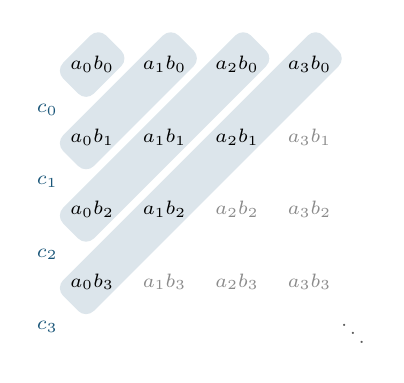
\begin{tikzpicture}[scale=0.92]
    % diagonal stripes along the anti-diagonals i + j = n
    \foreach \n in {0,1,2,3} {
      \pgfmathsetmacro{\cx}{\n/2}
      \pgfmathsetmacro{\hl}{0.707*\n + 0.42}
      \fill[defcolor!15, rounded corners=4pt,
            rotate around={45:(\cx,-\cx)}]
        (\cx-\hl, -\cx-0.3) rectangle (\cx+\hl, -\cx+0.3);
    }
    % grid of products: cells with i + j <= 3 belong to c_0 ... c_3
    \foreach \i in {0,1,2,3}
      \foreach \j in {0,1,2,3} {
        \pgfmathtruncatemacro{\s}{\i+\j}
        \ifnum\s>3
          \node[remcolor!70, font=\scriptsize] at (\i,-\j) {$a_{\i} b_{\j}$};
        \else
          \node[font=\scriptsize] at (\i,-\j) {$a_{\i} b_{\j}$};
        \fi
      }
    % stripe labels at the lower-left end of each diagonal
    \foreach \n in {0,1,2,3}
      \node[defcolor, font=\scriptsize\bfseries] at (-0.62,-\n-0.62) {$c_{\n}$};
    \node[remcolor, font=\scriptsize] at (3.6,-3.6) {$\ddots$};
  \end{tikzpicture}
  \end{center}

  \begin{hlbox}
    \vspace{-0.5em}
    \[
      c_n = \sum_{i+j=n} a_i b_j
      \qquad \text{(one \alert{anti-diagonal} per term)}
    \]
    \vspace{-1.2em}
  \end{hlbox}

  \note{
    This picture shows all the products you can form from the two series,
    arranged in an infinite grid. The columns are indexed by "i", the index
    of the "a" terms, and the rows are indexed by "j", the index of the "b"
    terms, so the cell in column "i" and row "j" contains the product "a"
    sub "i" times "b" sub "j". The shaded stripes run along the
    anti-diagonals of the grid, the sets of cells where "i" plus "j" is
    constant. Each stripe is labeled at its lower left end with the term it
    produces: the single corner cell gives "c" sub zero, the next stripe of
    two cells gives "c" sub one, the stripe of three cells gives "c" sub
    two, and so on. The grayed out cells in the lower right belong to later
    diagonals. Summing the Cauchy product series means sweeping out this
    grid one diagonal at a time. Now, does this product behave well? The
    next example gives a startling answer.
  }
\end{frame}
}

{
\usebackgroundtemplate{%
  
\includegraphics[width=\paperwidth,height=\paperheight,keepaspectratio=false]{chapter_03_bg_04.png}%
}
% =============================================================================
\section{A Product That Diverges}
% =============================================================================

\begin{frame}{Example 3.49 --- The Question}
  \begin{exblock}{Example 3.49: Setup}
    Let $A_n = \displaystyle\sum_{k=0}^{n} a_k$,\quad
    $B_n = \displaystyle\sum_{k=0}^{n} b_k$,\quad
    $C_n = \displaystyle\sum_{k=0}^{n} c_k$,\quad
    with $A_n \to A$, $B_n \to B$.
  \end{exblock}

  \vspace{0.5em}
  \begin{hlbox}
    \begin{itemize}
      \item It is \alert{not at all clear} that $C_n \to AB$,
        since $C_n \neq A_n B_n$
      \item The dependence of $\{C_n\}$ on $\{A_n\}$, $\{B_n\}$ is complicated
    \end{itemize}
  \end{hlbox}

  \note{
    Let's set up the question precisely. Capital "A" sub "n", capital "B"
    sub "n", and capital "C" sub "n" are the partial sums of the two given
    series and of their Cauchy product. Suppose the two given series
    converge, to "A" and "B". We would like the product series to converge
    to "A" times "B". But notice the first bullet: capital "C" sub "n" is
    not the product of capital "A" sub "n" and capital "B" sub "n". The
    product of the partial sums contains all products from a square block
    of the grid, while capital "C" sub "n" only sums the first few
    diagonals, which form a triangle. So the sequence result about products
    of limits does not apply, and the dependence of the product partial
    sums on the original ones is quite complicated. In fact, we will now
    show that the product of two convergent series may actually diverge.
  }
\end{frame}

\begin{frame}{Example 3.49 --- A Convergent Series}
  \begin{exblock}{The factor series}
    \[
      \sum_{n=0}^{\infty} \frac{(-1)^n}{\sqrt{n+1}}
      = 1 - \frac{1}{\sqrt{2}} + \frac{1}{\sqrt{3}} - \frac{1}{\sqrt{4}} + \cdots
    \]
    converges by the alternating series test (Theorem 3.43).
  \end{exblock}

  \vspace{0.5em}
  \begin{hlbox}
    \begin{itemize}
      \item Convergence is \alert{not absolute}:
        $\sum \frac{1}{\sqrt{n+1}}$ diverges
      \item We form the Cauchy product of this series \alert{with itself}
    \end{itemize}
  \end{hlbox}

  \note{
    Here is the series we will use, shown in the orange box. Its terms
    alternate in sign, and their absolute values, one over the square root
    of "n" plus one, decrease monotonically to zero. So Theorem 3.43, the
    alternating series test from the section on summation by parts, applies
    and the series converges. But notice the first bullet: the convergence
    is not absolute. The absolute values form essentially the series of one
    over the square root of "n", which diverges, since we know the series
    of one over "n" to the power "p" diverges whenever "p" is at most one.
    Keep that in mind for later. The plan now is to form the Cauchy product
    of this series with itself and watch what happens to the product terms.
  }
\end{frame}

\begin{frame}{Example 3.49 --- Squaring the Series}
  \begin{hlbox}
    The product terms are
    \begin{align*}
      \sum_{n=0}^{\infty} c_n &= 1
        - \left(\frac{1}{\sqrt{2}} + \frac{1}{\sqrt{2}}\right)
        + \left(\frac{1}{\sqrt{3}} + \frac{1}{\sqrt{2}\sqrt{2}} + \frac{1}{\sqrt{3}}\right) - \cdots
    \end{align*}
    so that
    \[
      c_n = (-1)^n \sum_{k=0}^{n} \frac{1}{\sqrt{(n-k+1)(k+1)}}
    \]
  \end{hlbox}

  \note{
    Let's compute the product terms. The first display shows the first few:
    the signs of the factors combine so that every product inside the
    "n"-th group has the same sign, namely negative one to the "n". For
    example, the group for "n" equal to one contains two copies of one over
    the square root of two, both negative. The general formula appears in
    the second display: "c" sub "n" is negative one to the "n", times the
    sum over "k" of one over the square root of the product of "n" minus
    "k" plus one and "k" plus one. There is no cancellation inside each
    "c" sub "n"; all "n" plus one summands reinforce each other. That is
    exactly what will sink the series. Next we estimate how big these terms
    are.
  }
\end{frame}

\begin{frame}{Example 3.49 --- The Terms Do Not Vanish}
  \begin{hlbox}
    Since
    $\;(n-k+1)(k+1) = \left(\frac{n}{2}+1\right)^2 - \left(\frac{n}{2}-k\right)^2
      \leq \left(\frac{n}{2}+1\right)^2$,
    \[
      |c_n| \;\geq\; \sum_{k=0}^{n} \frac{2}{n+2} \;=\; \boxed{\frac{2(n+1)}{n+2} \;\longrightarrow\; 2}
    \]
  \end{hlbox}

  \begin{center}
  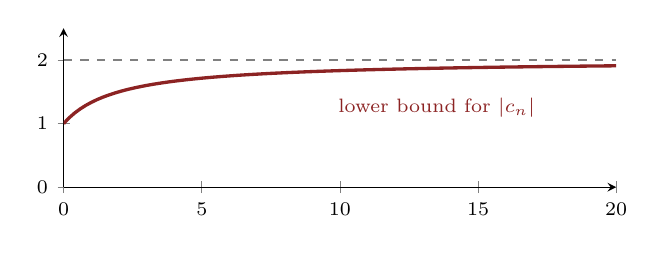
\begin{tikzpicture}
    \begin{axis}[width=8.6cm, height=3.6cm, xmin=0, xmax=20,
      ymin=0, ymax=2.5, axis lines=left,
      ytick={0,1,2}, label style={font=\scriptsize},
      tick label style={font=\scriptsize}]
      \addplot[gray, dashed, domain=0:20] {2};
      \addplot[thmcolor, very thick, domain=0:20, samples=100] {2*(x+1)/(x+2)};
      \node[thmcolor, font=\scriptsize] at (axis cs:13.5,1.25)
        {lower bound for $|c_n|$};
    \end{axis}
  \end{tikzpicture}
  \end{center}

  \hl{$c_n \not\to 0$, so $\Sigma c_n$ \alert{diverges} (Theorem 3.23)!}

  \note{
    Now the estimate. The identity at the top rewrites the product of "n"
    minus "k" plus one and "k" plus one by completing the square: it equals
    the square of "n" over two plus one, minus the square of "n" over two
    minus "k". Dropping the subtracted square only increases the value, so
    the product under the square root is at most the square of "n" over two
    plus one. Taking square roots, each denominator is at most "n" over two
    plus one, so each summand in "c" sub "n" is at least two over "n" plus
    two.
    Adding up the "n" plus one summands gives the boxed lower bound, two
    times "n" plus one, over "n" plus two. The graph shows this lower
    bound in red as "n" grows: it climbs toward the dashed line at height
    two, and never comes close to zero. But by Theorem 3.23, the terms of
    any convergent series must tend to zero. Here they do not, so the
    product series diverges. The product of two convergent series has
    diverged. Notice that both factors converged only nonabsolutely; the
    next theorem shows this is the only way such a failure can happen.
  }
\end{frame}
}

{
\usebackgroundtemplate{%
  
\includegraphics[width=\paperwidth,height=\paperheight,keepaspectratio=false]{chapter_03_bg_05.png}%
}
% =============================================================================
\section{Mertens' Theorem}
% =============================================================================

% --- Build 1/2 ---
\begin{frame}{Theorem 3.50 (Mertens)}
  \begin{thmblock}{Theorem 3.50: Hypotheses}
    Suppose
    \begin{enumerate}
      \item[(a)] $\sum_{n=0}^{\infty} a_n$ converges \alert{absolutely},
      \item[(b)] $\sum_{n=0}^{\infty} a_n = A$,
      \item[(c)] $\sum_{n=0}^{\infty} b_n = B$,
      \item[(d)] $c_n = \sum_{k=0}^{n} a_k b_{n-k}$
        \quad $(n = 0, 1, 2, \dots)$.
    \end{enumerate}
  \end{thmblock}

  \note{
    Here is the theorem of Mertens, with its four hypotheses listed in the
    red box. Hypothesis "a" is the crucial one: the first series converges
    absolutely. Hypothesis "b" names its sum "A", hypothesis "c" says the
    second series converges with sum "B", and notice that for the second
    series we ask only for plain convergence, nothing more. Hypothesis "d"
    just recalls the definition of the Cauchy product terms "c" sub "n".
    So the setup is deliberately asymmetric: one factor is strong,
    absolutely convergent, while the other factor can be as fragile as the
    alternating series from the previous example. Next, the conclusion.
  }
\end{frame}

% --- Build 2/2 ---
\begin{frame}{Theorem 3.50 (Mertens)}
  \begin{thmblock}{Theorem 3.50: Hypotheses}
    Suppose
    \begin{enumerate}
      \item[(a)] $\sum_{n=0}^{\infty} a_n$ converges \alert{absolutely},
      \item[(b)] $\sum_{n=0}^{\infty} a_n = A$,
      \item[(c)] $\sum_{n=0}^{\infty} b_n = B$,
      \item[(d)] $c_n = \sum_{k=0}^{n} a_k b_{n-k}$
        \quad $(n = 0, 1, 2, \dots)$.
    \end{enumerate}
  \end{thmblock}

  \begin{thmblock}{Conclusion}
    \vspace{-0.4em}
    \[
      \sum_{n=0}^{\infty} c_n = AB
    \]
    \vspace{-1.2em}
  \end{thmblock}

  \note{
    And here is the conclusion: the Cauchy product series converges, and
    its sum is exactly "A" times "B". In words: the product of two
    convergent series converges, and to the right value, provided at least
    one of the two series converges absolutely. Compare this with Example
    3.49. There, both factors converged only nonabsolutely, and the product
    fell apart. Mertens' theorem tells us that one absolutely convergent
    factor is enough to prevent that disaster. Before diving into the
    proof, let's lay out the strategy.
  }
\end{frame}

\begin{frame}{Proof Strategy: Theorem 3.50}
  \begin{hlbox}
    \textbf{Goal:} show $C_n = \sum_{k=0}^{n} c_k \to AB$.

    \vspace{0.6em}
    \textbf{Approach:}
    \begin{enumerate}
      \item Regroup $C_n$ as a combination of the $a_k$ and the
        partial sums $B_k$
      \item Split off the \alert{main term} $A_n B$ (which $\to AB$)
        plus a remainder $\gamma_n$
      \item Show $\gamma_n \to 0$: split it at a cutoff $N$ where
        $B_k$ is close to $B$
      \item Control the tail using $\alpha = \Sigma |a_n|$ ---
        \alert{this is where absolute convergence enters}
    \end{enumerate}
  \end{hlbox}

  \note{
    Here is the road map, in four steps. First, we regroup the product
    partial sum capital "C" sub "n" so that it is expressed through the
    terms "a" sub "k" of the strong series and the partial sums capital "B"
    sub "k" of the weak one. Second, we split off a main term, capital "A"
    sub "n" times "B", which clearly converges to "A" times "B", plus a
    remainder gamma sub "n". Everything then reduces to showing that the
    remainder tends to zero. Third, to do that, we cut the remainder into
    two pieces at an index "N" beyond which the partial sums capital "B"
    sub "k" are within epsilon of "B". Fourth, the piece with small betas
    is controlled by alpha, the sum of the absolute values of the "a" sub
    "n". This is precisely where absolute convergence earns its keep. With
    the plan in hand, let's carry out step one.
  }
\end{frame}

\begin{frame}{Proof of Theorem 3.50 --- Step 1: Regrouping $C_n$}
  \begin{proofblock}{Step 1: Express $C_n$ via the partial sums $B_k$}
    Put $A_n = \sum_{k=0}^{n} a_k$,\quad $B_n = \sum_{k=0}^{n} b_k$,\quad
    $C_n = \sum_{k=0}^{n} c_k$. Then
    \begin{align*}
      C_n &= a_0 b_0 + (a_0 b_1 + a_1 b_0) + \cdots
             + (a_0 b_n + a_1 b_{n-1} + \cdots + a_n b_0) \\
          &= a_0 B_n + a_1 B_{n-1} + \cdots + a_n B_0
    \end{align*}
  \end{proofblock}

  \vspace{0.4em}
  \hl{\textbf{Technique:} regroup by the \alert{$a$-factor} instead of by diagonal.}

  \note{
    Step one is a regrouping trick. Write out capital "C" sub "n" as the
    sum of all the diagonal groups, as in the first line. Now, instead of
    reading this triangle of products diagonal by diagonal, collect all
    the products that share the same "a"-factor. The terms containing "a"
    sub zero are "a" sub zero times "b" sub zero through "b" sub "n", which
    add up to "a" sub zero times capital "B" sub "n". The terms containing
    "a" sub one pair with "b" sub zero through "b" sub "n" minus one,
    giving "a" sub one times capital "B" sub "n" minus one. Continuing,
    we get the second line: a convolution of the "a" terms with the partial
    sums of the "b" series. This expresses the complicated object through
    things we understand. Next we feed in what we know about those partial
    sums.
  }
\end{frame}

\begin{frame}{Proof of Theorem 3.50 --- Step 2: Main Term + Remainder}
  \begin{proofblock}{Step 2: Split off $A_n B$}
    Put $\beta_n = B_n - B$ (so $\beta_n \to 0$). Then
    \begin{align*}
      C_n &= a_0(B + \beta_n) + a_1(B + \beta_{n-1}) + \cdots + a_n(B + \beta_0) \\
          &= A_n B + \underbrace{a_0 \beta_n + a_1 \beta_{n-1} + \cdots
             + a_n \beta_0}_{=\;\gamma_n}
    \end{align*}
    Since $A_n B \to AB$, it suffices to show
    \begin{equation}
      \lim_{n \to \infty} \gamma_n = 0. \tag{21}
    \end{equation}
  \end{proofblock}

  \note{
    Step two isolates the main term. Define beta sub "n" as the error of
    the "n"-th partial sum of the "b" series, capital "B" sub "n" minus
    "B". By hypothesis "c", these errors tend to zero. Substituting "B"
    plus the error into each partial sum in our formula and expanding, the
    "B" terms collect into capital "A" sub "n" times "B", and the leftovers
    form the quantity gamma sub "n", the convolution of the "a" terms with
    the errors beta. Now the main term capital "A" sub "n" times "B"
    converges to "A" times "B", which is exactly the value we want. So
    everything boils down to equation 21: the remainder gamma sub "n" must
    tend to zero. Intuitively this is plausible, since the betas tend to
    zero, but the number of summands in gamma sub "n" grows with "n", so we
    need to be careful. That is the content of the next step.
  }
\end{frame}

\begin{frame}{Proof of Theorem 3.50 --- Step 3: Splitting $\gamma_n$}
  \begin{proofblock}{Step 3: Cut at a threshold $N$}
    Put $\alpha = \sum_{n=0}^{\infty} |a_n|$ \quad
    [\alert{here we use (a)!}]

    Given $\varepsilon > 0$: since $\beta_n \to 0$, choose $N$ with
    $|\beta_n| \leq \varepsilon$ for $n \geq N$. Then
    \begin{align*}
      |\gamma_n|
        &\leq |\beta_0 a_n + \cdots + \beta_N a_{n-N}|
          + |\beta_{N+1} a_{n-N-1} + \cdots + \beta_n a_0| \\
        &\leq |\beta_0 a_n + \cdots + \beta_N a_{n-N}| + \varepsilon \alpha
    \end{align*}
  \end{proofblock}

  \note{
    Step three is the heart of the proof. First define alpha as the sum of
    the absolute values of the "a" sub "n". This number is finite precisely
    because of hypothesis "a"; this is the one and only place where
    absolute convergence is used. Now let epsilon be given. Since the betas
    tend to zero, we can choose a threshold "N" beyond which every beta has
    absolute value at most epsilon. Split gamma sub "n" into two pieces, as
    in the display: the early betas, beta sub zero through beta sub "N",
    each multiplied by a late "a" term, and the late betas, which come
    multiplied by various "a" terms. For the second piece, each beta is at
    most epsilon, and the sum of the absolute values of the accompanying
    "a" factors is at most alpha. So the second piece is at most epsilon
    times alpha, a quantity we control. The first piece still depends on
    "n", and the final step deals with it.
  }
\end{frame}

\begin{frame}{Proof of Theorem 3.50 --- Step 4: Letting $n \to \infty$}
  \begin{proofblock}{Step 4: The first piece dies out}
    Keep $N$ \alert{fixed}, let $n \to \infty$. Since $a_k \to 0$
    as $k \to \infty$,
    \[
      |\beta_0 a_n + \cdots + \beta_N a_{n-N}| \to 0
      \quad\Longrightarrow\quad
      \limsup_{n \to \infty} |\gamma_n| \leq \varepsilon \alpha.
    \]
    Since $\varepsilon$ is arbitrary, (21) follows. \hfill $\blacksquare$
  \end{proofblock}

  \vspace{0.3em}
  \begin{hlbox}
    \centering
    $\boxed{\;\displaystyle\sum_{n=0}^{\infty} c_n = AB\;}$
  \end{hlbox}

  \note{
    Step four finishes the job. The first piece consists of a fixed number
    of summands, namely "N" plus one of them, with fixed coefficients beta
    sub zero through beta sub "N". The "a" factors in this piece have
    indices "n" minus "N" through "n", which march off to infinity as "n"
    grows, and the terms of a convergent series tend to zero, so each "a"
    factor tends to zero. A fixed finite sum of terms each tending to zero
    tends to zero. Therefore the limit superior of the absolute value of
    gamma sub "n" is at most epsilon times alpha. But epsilon was an
    arbitrary positive number, and alpha is a fixed finite constant, so the
    limit superior must be zero, which is exactly equation 21. The
    remainder vanishes, the main term gives "A" times "B", and the boxed
    conclusion follows: the Cauchy product converges to "A" times "B".
    One natural question remains, and Abel answered it.
  }
\end{frame}
}

{
\usebackgroundtemplate{%
  
\includegraphics[width=\paperwidth,height=\paperheight,keepaspectratio=false]{chapter_03_bg_06.png}%
}
% =============================================================================
\section{Abel's Theorem}
% =============================================================================

\begin{frame}{Theorem 3.51 (Abel)}
  \begin{thmblock}{Theorem 3.51}
    If the series $\Sigma a_n$, $\Sigma b_n$, $\Sigma c_n$ converge to
    $A$, $B$, $C$, and $c_n = a_0 b_n + \cdots + a_n b_0$, then
    \[
      C = AB.
    \]
  \end{thmblock}

  \vspace{0.5em}
  \begin{hlbox}
    \begin{itemize}
      \item \alert{No} absolute convergence is assumed!
      \item If the Cauchy product converges, it converges
        to the \alert{right value}
      \item Proof deferred: it uses the continuity of power series 
        (Chapter 8)
    \end{itemize}
  \end{hlbox}

  \note{
    Here is the last result of the section, due to Abel. Suppose all three
    series converge: the two factors, with sums "A" and "B", and their
    Cauchy product, with sum "C". Then "C" must equal "A" times "B". Look
    at the bullets below the box. First, no assumption of absolute
    convergence is made anywhere. Second, this answers the remaining
    question: the Cauchy product of two convergent series might diverge, as
    we saw, but if it happens to converge, it cannot converge to the wrong
    value. Third, we do not prove this theorem now. A simple proof depends
    on the continuity of power series, a tool we will only develop in
    Chapter 8, so the proof will come right after Theorem 8.2. Let's
    summarize what we have learned.
  }
\end{frame}
}

{
\usebackgroundtemplate{%
  
\includegraphics[width=\paperwidth,height=\paperheight,keepaspectratio=false]{chapter_03_bg_07.png}%
}
% =============================================================================
\section{Summary}
% =============================================================================

% --- Build 1/3 ---
\begin{frame}{Summary}
  \begin{hlbox}
    \textbf{Key takeaways from this section:}
    \begin{itemize}
      \item \textbf{Addition (3.47):} convergent series add term by term:
        $\Sigma(a_n + b_n) = A + B$, $\Sigma c a_n = cA$
    \end{itemize}
  \end{hlbox}

  \note{
    Let's review what we covered. First, addition is completely
    unproblematic. Theorem 3.47 says that two convergent series may be
    added term by term, and the result converges to the sum of the two
    sums; likewise, a constant factor can be pulled out of a convergent
    series. The proof was a one-liner using the arithmetic of limits.
    Next, the product.
  }
\end{frame}

% --- Build 2/3 ---
\begin{frame}{Summary}
  \begin{hlbox}
    \textbf{Key takeaways from this section:}
    \begin{itemize}
      \item \textbf{Addition (3.47):} convergent series add term by term:
        $\Sigma(a_n + b_n) = A + B$, $\Sigma c a_n = cA$
      \item \textbf{Cauchy product (3.48):} $c_n = \sum_{k=0}^n a_k b_{n-k}$,
        motivated by multiplying power series
      \item \textbf{Danger (3.49):} the product of two \alert{nonabsolutely}
        convergent series can \alert{diverge}
    \end{itemize}
  \end{hlbox}

  \note{
    Second, multiplication required a definition: the Cauchy product, whose
    "n"-th term collects all products of terms whose indices add to "n".
    The definition is exactly what multiplying power series and setting "z"
    equal to one suggests. Third, the warning of Example 3.49: the Cauchy
    product of the alternating series of one over the square root of "n"
    plus one with itself has terms that stay near size two instead of
    tending to zero, so the product of two convergent series can diverge.
    Finally, the two positive results.
  }
\end{frame}

% --- Build 3/3 ---
\begin{frame}{Summary}
  \begin{hlbox}
    \textbf{Key takeaways from this section:}
    \begin{itemize}
      \item \textbf{Addition (3.47):} convergent series add term by term:
        $\Sigma(a_n + b_n) = A + B$, $\Sigma c a_n = cA$
      \item \textbf{Cauchy product (3.48):} $c_n = \sum_{k=0}^n a_k b_{n-k}$,
        motivated by multiplying power series
      \item \textbf{Danger (3.49):} the product of two \alert{nonabsolutely}
        convergent series can \alert{diverge}
      \item \textbf{Mertens (3.50):} one \alert{absolutely} convergent factor
        $\Rightarrow$ $\Sigma c_n = AB$;\;
        \textbf{Abel (3.51):} if $\Sigma c_n$ converges, its sum is $AB$
    \end{itemize}

    \vspace{0.3em}
    \textbf{Coming up next:} Rearrangements --- can reordering
    change the sum?
  \end{hlbox}

  \note{
    The last bullet collects the two positive results. Mertens' theorem:
    if at least one of the two factors converges absolutely, the Cauchy
    product converges to "A" times "B"; the proof split the product partial
    sums into a main term plus a convolution remainder, and absolute
    convergence tamed the remainder. And Abel's theorem: with no absolute
    convergence at all, if the Cauchy product happens to converge, its sum
    is necessarily "A" times "B"; the proof waits until Chapter 8. Once
    again absolute convergence was the dividing line between good and bad
    behavior. In the next section we will see this even more dramatically:
    we study rearrangements, and discover that reordering the terms of a
    nonabsolutely convergent series can change its sum to anything we like,
    while absolutely convergent series are immune to reordering. See you
    there.
  }
\end{frame}
}

\end{document}
